\documentclass[t]{beamer}
\usetheme{amcg}
\usepackage{hyperref}
\hypersetup{
    colorlinks=true,
    linkcolor=cyan,
    urlcolor=cyan
}
\usepackage{mathptmx}
\usepackage{helvet}
\newcommand\TILDE{\char`\~}
\usepackage{listings}
\setbeamertemplate{navigation symbols}{}

\author[Alexandros Avdis]{Applied Modelling and Computation Group\\[15pt]Alexandros Avdis}

\institute{Department of Earth Science and Engineering, Imperial College London}

\date{5-7 November 2014}
\title[Meshing]{Meshing}
\subtitle[]{Fluidity training workshop}

\setbeamersize{text margin left=0.3in}
\setbeamersize{text margin right=0.3in}

\begin{document}
{
\setbeamertemplate{footline}
{%
\begin{beamercolorbox}[ht=.35cm,dp=0.2cm,wd=\textwidth,leftskip=.3cm]{author in head/foot}%
        \begin{minipage}[c]{5cm}%
        \usebeamerfont{author in head/foot}
        \end{minipage}\hfill% 
        \begin{minipage}{6cm}
        \hfill\includegraphics[height=.5cm]{AMCGFlow-long}
        \end{minipage}
\end{beamercolorbox}%
}
\begin{frame}
\titlepage
\end{frame}
}

\begin{frame}{Tutorial overview~~~~~~~}
\begin{columns}[l]

\column{2.8in}
  \begin{itemize}
     \item What is a mesh.\\[17pt]
     \item What is Gmsh.\\[17pt]
     \item Viewing and meshing a 3--D geometry.\\[17pt]
     \item Generating and meshing a 2--D geometry.\\[17pt]
     \item Meshing realistic domains.
  \end{itemize}

\column{1.75in}
\vspace{-0.9in}
\begin{figure}[htbp!]
 \centering
  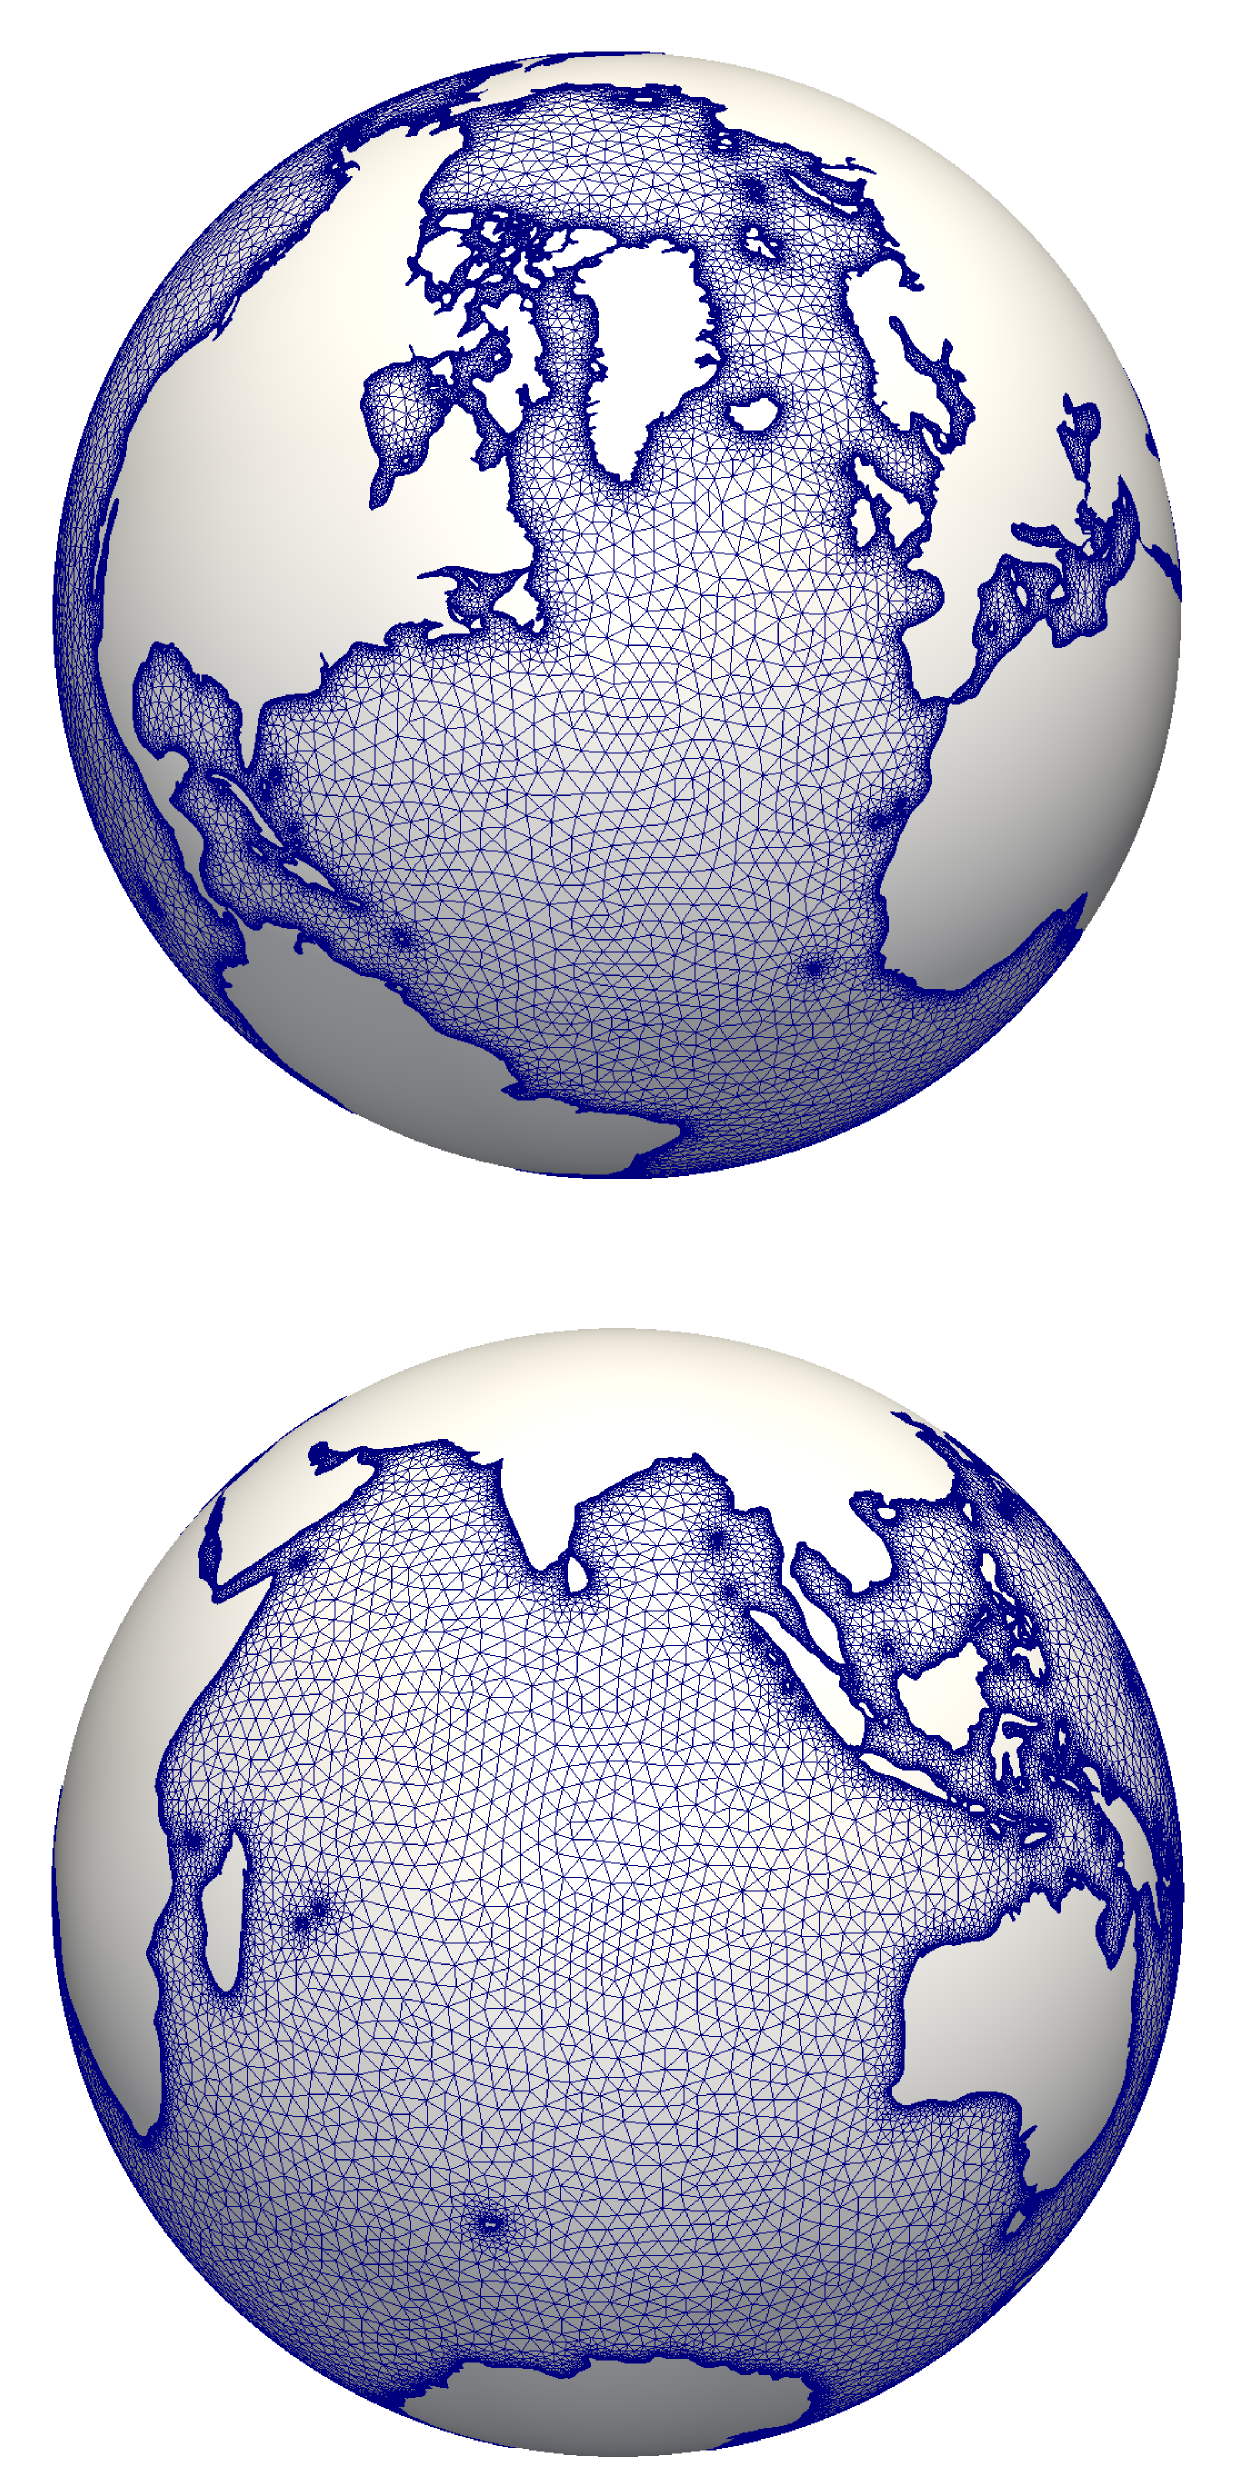
\includegraphics[width=1.0\textwidth]{../figures/globe_mesh}
\end{figure}
\end{columns}
\end{frame}

\begin{frame}{but, before we start...}
  \begin{itemize}
      \item This is a hands--on session, we need to do a bit of house--keeping.
      \vspace{10pt}
      \item Open a new terminal (Ctrl$+$Alt$+$t) :
      \begin{itemize}
         \item[$\circ$] We will be using this terminal throughout this tutorial.
         \item[\$] \emph{text} signifies commands to be typed into the terminal.
         \item[\$] \emph{mkdir mesh} \\to create a directory for this tutorial
         \item[\$] \emph{cd mesh} \\to ``enter'' the newly created directory
      \end{itemize}
      \vspace{10pt}
      \item Fetch \& open a copy of the present slides:
      \begin{itemize}
         \item[$\circ$] For the duration of the training event slides are on \emph{scratch}
         \item[\$] \emph{cp /scratch/gmsh\_tutorial\_presentation.pdf .} 
         \item[\$] \emph{evince gmsh\_tutorial\_presentation.pdf \&} \\ \hspace{10pt} The ampersand is important.
      \end{itemize}
  \end{itemize}
\end{frame}

\begin{frame}{A bit more house--keeping.}
  \begin{itemize}
     \item Keep the slides open in a window.
     \begin{itemize}
         \item[$\circ$] You can copy--paste lengthy commands \& statements.
         \item[$\circ$] You will be asked to click on links in the slides.
         \item[$\circ$] Feel free to progress at a faster pace than the speaker.
         \item[$\circ$] Feel free to put your hand up and ask for help!
     \end{itemize}
     \vspace{10pt}
     \item The slides, as well as a more detailed tutorial, are freely available.\\
     \begin{itemize}
         \item[$\circ$] You can download via Figshare:
         \item[$\circ$] \href{http://figshare.com/s/0dbd16a2635b11e4a71206ec4b8d1f61}{slides}
         \item[$\circ$] \url{tutorial document}
     \end{itemize}
  \end{itemize}
\end{frame}

\begin{frame}{What is a mesh?}
\only<1->{
A mesh can be qualitatively thought of as the tessellation of a domain $\Omega$ into a set of
non-overlapping sub-domains $\omega_i$:
}
\only<1>{
\begin{align}
\Omega &= \cup \left\{ \omega_i \left| i=1,2,\ldots ele \right. \right\} \nonumber \\
\label{eqn:tessalation_definition} \\
0 &= \cap \left\{ \omega_i \left| i=1,2,\ldots ele \right. \right\} \nonumber
\end{align}
where $ele$ is the number of elements in the tessellation.
}
\only<2>{
\begin{figure}[htbp!]
 \centering
  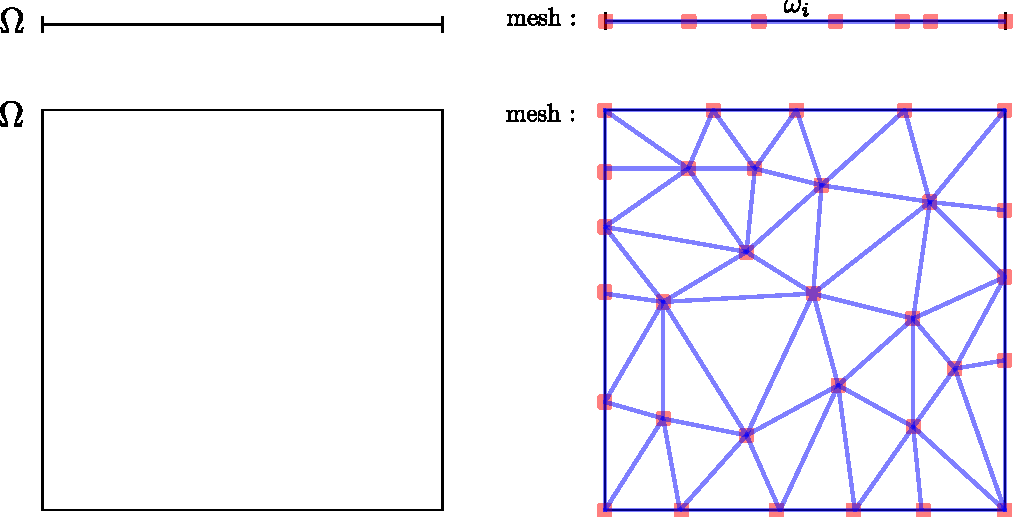
\includegraphics[width=0.85\textwidth]{../figures/1d_2d_mesh_examples}
\end{figure}
}
\end{frame}


\begin{frame}{What is Gmsh?}
\begin{itemize}
\item It is the role of the mesh (or grid) generator to scatter the points and generate the mesh, whilst ensuring high quality elements.
\item Gmsh is a \emph{``3D finite element grid generator with a build-in CAD engine and post-processor. Its design goal is to provide a fast, light and user-friendly meshing tool with parametric input and advanced visualization capabilities.''}\footnote{from \url{http://www.geuz.org/gmsh/}}. Furthermore, Gmsh can be used as a 1--, 2-- and 3-- dimensional mesh generator for use with the Fluidity CFD code.
\item Not the only mesh generator that can be used with Fluidity.
\begin{itemize}
   \item Fluidity can also read meshes in ExodusII format.
\end{itemize}
\item Distributed under the GNU General Public License, available for Linux, Windows and Mac OS.
\end{itemize}
\end{frame}

\begin{frame}{Fetching an example}
\begin{itemize}
   \item Lets fetch a Gmsh file and open it.
   \item Download a simple example file:
   \begin{itemize}
      \item[$\circ$] Point your browser to \href{http://figshare.com/s/b0936b565f8211e4aee906ec4b8d1f61}{here}
      \item[$\circ$] Look at the file contents, it is a geometry description.
      \item[$\circ$] Click on ``Download''.
   \end{itemize}\vspace{10pt}
   \item Go back to your terminal
   \begin{itemize}
      \item[\$] \emph{mv \$HOME/Downloads/annulus.geo .} \\to move the downloaded file into the new directory
   \end{itemize}
\end{itemize}
\end{frame}

\begin{frame}{Starting Gmsh}
  \begin{itemize} 
     \item Open the file, with Gmsh:
     \begin{itemize} 
         \item[\$] \emph{gmsh annulus.geo \&} \\ \hspace{10pt} The ampersand is important.
     \end{itemize} 
     \item The Gmsh window is composed of two panels:
  \end{itemize}
\vspace{-15pt}
\begin{columns}[l]
\column{2.3in}
  \begin{itemize} 
        \item[$\circ$] A menu panel, a tree--like structure (left).
        \item[$\circ$] The Graphic area (larger, right).
        \item[$\circ$] A status bar at the bottom.
  \end{itemize}
\column{2.2in}
\vspace{-5pt}
\begin{figure}[htbp!]
 \centering
  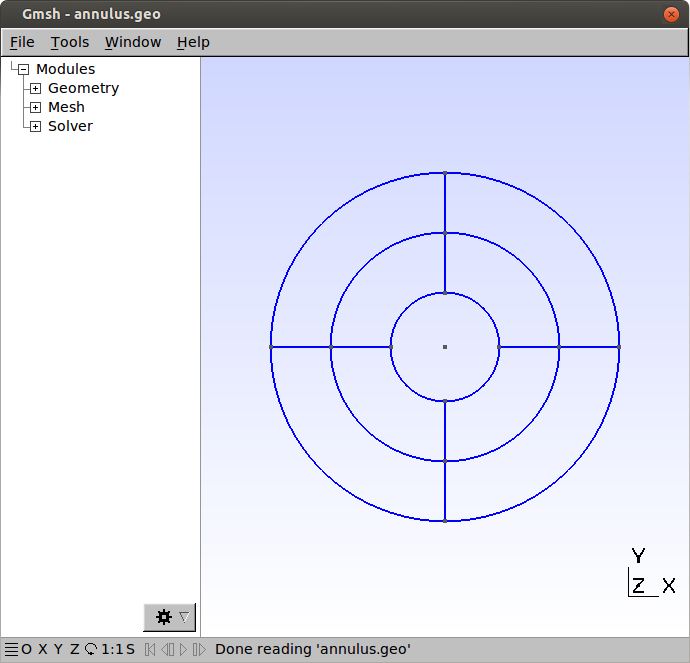
\includegraphics[width=1.0\textwidth]{../figures/annulus1}
  \label{fig:annulus1}
\end{figure}
\end{columns}
\end{frame}

\begin{frame}{Navigating menus.}
   \begin{itemize}
     \item Gmsh's architecture is centred around four modules, this is reflected in the menu panel.\\[10pt]
     \item The menu panel can be used to switch between the different modules.\\[10pt]
     \begin{enumerate}
       \item Geometry : For defining domain geometry.
       \item Mesh : For building the mesh.
       \item Solver.
       \item Post--Processing : More visible in older versions of Gmsh.
     \end{enumerate}
   \end{itemize}
\end{frame}

\begin{frame}{Manipulating the view}
\begin{itemize}
\item Panning : Hold right button down and move cursor.
\item Zooming : Scroll or hold middle button down and move cursor.
\item Rotating : Hold left button down and move cursor.
\item \emph{Practical :} Try modifying the view.
\end{itemize}
\end{frame}

\begin{frame}{Meshing and saving the mesh}
\begin{itemize}
\item Mesh the annulus
\begin{itemize}
  \item[$\circ$] \lstinline{Mesh > 3D}
  \item[$\circ$] Once again, try modifying the view.
\end{itemize}
\vspace{5pt}
\item To save the mesh click on File (menu window) and select Save Mesh.
\begin{itemize}
  \item[$\circ$] This creates a file ``annulus.msh'', storing the mesh.
\end{itemize}
\vspace{5pt}
\item More information on the annulus is available in the tutorial document fetched earlier.
\begin{itemize}
  \item[$\circ$] Including instructions how to build the geometry.
\end{itemize}
\end{itemize}
\end{frame}

\begin{frame}{The various files}
   \begin{itemize}
      \item annulus.geo : Stores the geometry as an ASCII script file.
      \begin{itemize}
         \item[$\circ$] You have already seen the contents, when downloading.
         \item[\$] \emph{cat annulus.geo} \\ \hspace{10pt} To list the file lines (catenate) in your terminal
         \item[$\circ$] Possible to write this file from scratch with a text editor.
         \item[$\circ$] Possible to use the Gmsh GUI to create this file.
      \end{itemize}\vspace{10pt}
      \item annulus.msh : Stores the mesh
      \begin{itemize}
         \item[$\circ$] Also contains tags (numerical ID) on element vertices, edges and faces that we can use to assign boundary conditions.
         \item[$\circ$] Can be ASCII or binary.
         \item[\$] \emph{cat annulus.msh} \\ \hspace{10pt} The file we generated here is ASCII
      \end{itemize}
   \end{itemize}
\end{frame}

\begin{frame}{Mesh file formats}
   \begin{itemize}
      \item Fluidity can read meshes in gmsh format.\vspace{10pt}
      \item Fluidity can also read meshes in triangle format.
      \begin{itemize}
         \item[$\circ$] The gmsh2triangle utility is part of the Fluidity distribution and can convert gmsh to triangle format:
         \item[\$] \emph{gmsh2triangle annulus.msh} \\ \hspace{10pt} Generates annulus.ele, annnulus.face, annulus.node
         \item[\$] \emph{ls -l} \\ \hspace{10pt} to list the files.
         \item[\$] \emph{gmsh2triangle} \\ \hspace{10pt} Shows usage and options.\vspace{10pt}
      \end{itemize}
      \item Fluidity can also read meshes in ExodusII format.\vspace{10pt}
      \item Work is on--going on PETSc DMPlex capability.
   \end{itemize}
\end{frame}

\begin{frame}{Gyre example: Aim}

\begin{itemize}
    \item To generate a 2--D mesh on a $1,000$km $\times 1,000$km square.
    \item Using the Gmsh GUI.
    \item Typical element size (edge length): $20$km.
    \item Mesh will be used in subsequent simulations/examples.
\end{itemize}

\begin{figure}[htbp]
 \centering
  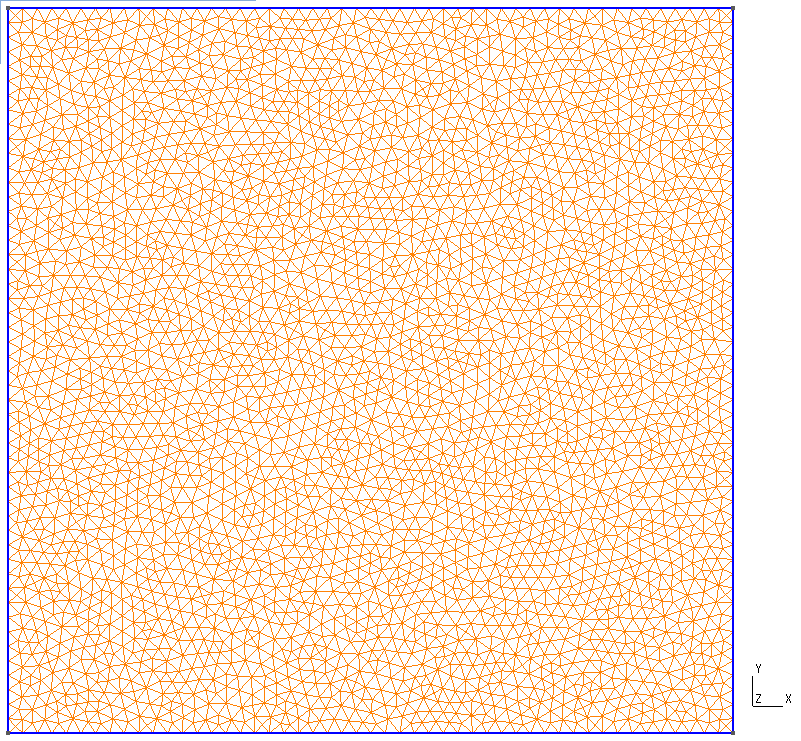
\includegraphics[width=0.5\textwidth]{../figures/2d-example-mesh}
\end{figure}

\end{frame}


\begin{frame}{Gyre example: Getting started}
    \begin{itemize}
        \item Close your existing Gmsh instance.
        \item Download the solution file, to help you \& tutors trace mistakes.
        \begin{itemize}
            \item[$\circ$] Download from \href{http://figshare.com/s/85271e16603d11e4840b06ec4bbcf141}{here}
            \item[\$] \emph{mv \$HOME/Downloads/gyre-example.geo .}
        \end{itemize}
        \item Open a new Gmsh instance, on a new file:
        \begin{itemize}
            \item[\$] \emph{gmsh gyre.geo \&} \\ \hspace{10pt} The ampersand is important.\vspace{10pt}
        \end{itemize}
    \end{itemize}
    We proceed by defining:
    \begin{enumerate}
        \item Points
        \item Lines
        \item Surfaces
        \item in 3D cases, volumes
    \end{enumerate}
\end{frame}

\begin{frame}{Gyre example: Creating points}
  \begin{itemize}
  \item \lstinline{Geometry > Elementary Entities > Add > Point}\\[4pt]
  \item The \emph{Contextual Geometry Definitions} window will appear.\\[4pt]
  \item Enter the point coordinates and click ``Add''.\\[4pt]
  \begin{itemize}
    \item[$\circ$] Do not move cursor outside \emph{Contextual Geometry Definitions} window while entering coordinates! Hold shift down if you have to.\\[4pt]
    \item[$\circ$] Always look at the instructions shown in the graphic window.\\[4pt]
    \item[$\circ$] Point 1: \emph{[ 0.0\ \ ,  0.0\ \ ,  0.0]}, Prescribed mesh element size \emph{2e4}\\[5pt]
    \item[$\circ$] Point 2: \emph{[ 0.0\ \ ,  1.e6,\ \ 0.0]}, Prescribed mesh element size \emph{2e4}\\[5pt]
    \item[$\circ$] Point 3: \emph{[ 1.e6, 1.e6,\ \ 0.0]}, Prescribed mesh element size \emph{2e4}\\[5pt]
    \item[$\circ$] Point 4: \emph{[ 1.e6, 0.0\ \ ,  0.0]}, Prescribed mesh element size \emph{2e4}\\[5pt]
    \end{itemize}
  \item Press `q' and close Contextual Geometry Definitions window.
  \end{itemize}
\end{frame}

\begin{frame}{Gyre example: Creating lines}
\begin{itemize}
\item Geometry $>$ Elementary Entities $>$ Add $>$ Straight Line
\begin{itemize}
\item[$\circ$] Draw a line between two points by selecting the points.
\item[$\circ$] Join points \emph{(1,2)}, \emph{(2,3)}, \emph{(3,4)}, \emph{(4,1)}
\item[$\circ$] Once all lines are drawn, press `q'
\item[$\circ$] Always look at the instructions shown in the graphic panel.
\end{itemize}
\end{itemize}
\begin{figure}[htbp]
 \centering
  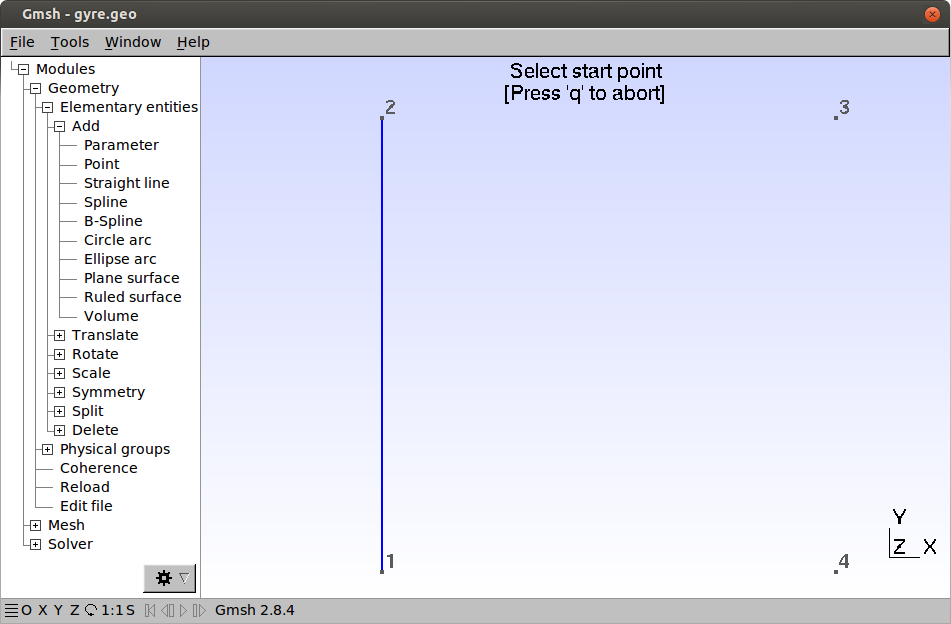
\includegraphics[width=0.65\textwidth]{../figures/Gmsh_drawing_lines.png}
\end{figure}
\end{frame}

\begin{frame}{Gyre example: Declaring a plane surface.}
\begin{itemize}
\item Geometry $>$ Elementary Entities $>$ Add $>$ Plane Surface
\item Click on any of the sides, all sides will be highlighted.
\item Press `e' then `q'.
\item Gmsh will highlight the surface with grey, dash-lines.
\end{itemize}
\begin{figure}[htbp]
 \centering
  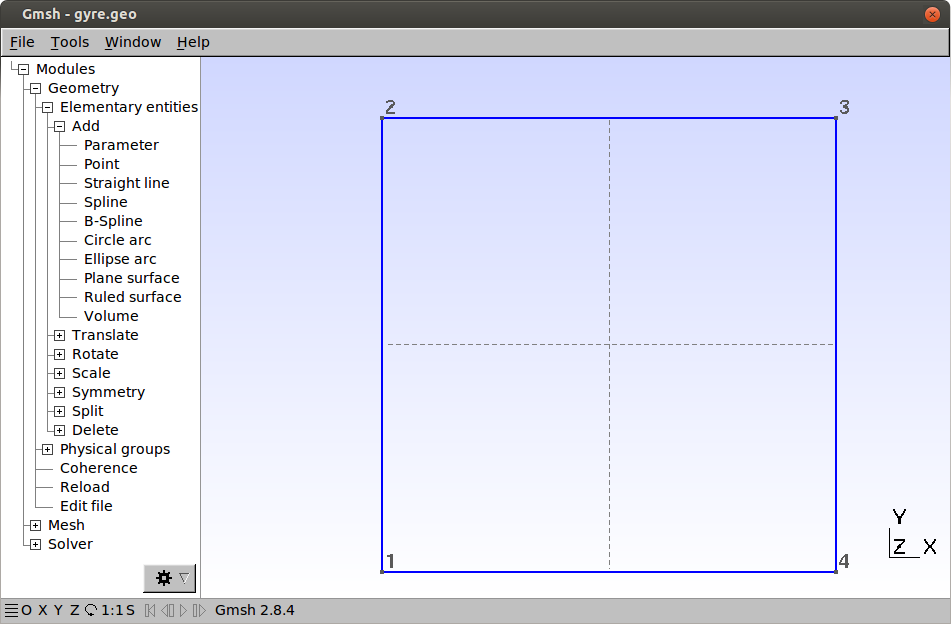
\includegraphics[width=0.65\textwidth]{../figures/2d-example-surface}
\end{figure}
\end{frame}

\begin{frame}{Gyre example: Declaring physical groups.}
In order to specify regions and boundaries in Fluidity, they must first be defined as ``Physical Groups'' in Gmsh:\\[15pt]

\begin{itemize}
   \item Assign ``Physical Line'' ID's to the domain boundaries.
   \begin{itemize}
      \item[$\circ$] \lstinline{Geometry > Physical Groups > Add > Line}
      \item[$\circ$] Select \emph{bottom} side and press `e'.
      \item[$\circ$] Select \emph{right} side and press `e'.
      \item[$\circ$] Select \emph{top} side and press `e'.
      \item[$\circ$] Select \emph{left} side and press `e'.
      \item[$\circ$] Once you have done all sides press `q'.\\[15pt]
   \end{itemize}
   \item Assign ``Physical Surface'' ID to the plane surface.
   \begin{itemize}
      \item[$\circ$] \lstinline{Geometry > Physical Groups > Add > Surface}
      \item[$\circ$] Select the highlighted surface: Click on the grey dash lines.
      \item[$\circ$] Press `e' then `q'.
   \end{itemize}
\end{itemize}
\end{frame}

\begin{frame}{Gyre example: Producing a mesh}
   \begin{itemize}
      \item Produce a 2--D mesh: \lstinline{Mesh > 2D}
      \item Save the mesh: Click on File and select ``Save Mesh''.
      \item Convert to triangle format:
      \begin{itemize}
          \item[\$]\emph{gmsh2triangle -2 gyre.msh}
      \end{itemize}
   \end{itemize}
\begin{figure}[htbp]
 \centering
  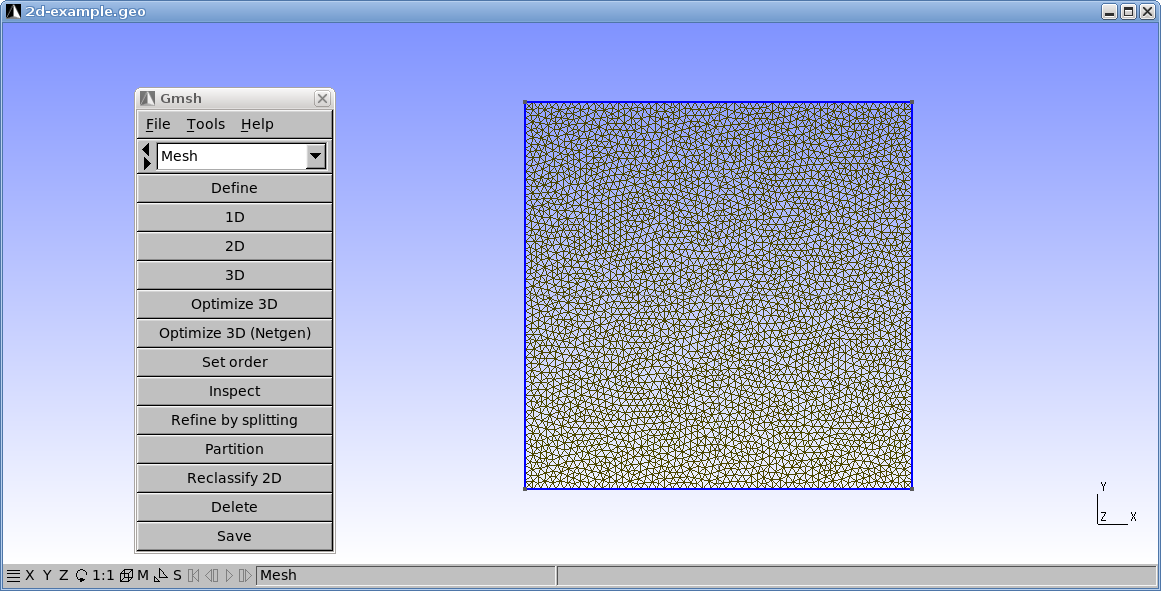
\includegraphics[width=0.65\textwidth]{../figures/2d-example-Gmsh-mesh}
  \label{fig:shot16}
\end{figure}
\end{frame}

\begin{frame}{Meshes for realistic ocean domains \& Fluidity}
\begin{itemize}
    \item Mesh is constructed on a reference surface.
    \begin{itemize}
        \item[$\circ$] A spherical shell, Earth's surface geoid.
        \item[$\circ$] A flat surface, a chartographic projection datum (e.g. a UTM zone).
    \end{itemize}
    \item User can choose to set--up 2D or 3D simulations
    \begin{itemize}
        \item[$\circ$] 2D, suitable for regional shallow water (not currently on--the--sphere).
        \item[$\circ$] In 3D no need  to do three-dimensional mesh generation.
        \item[$\circ$] Mesh is ``vertically extruded'' within Fluidity.
    \end{itemize}
\end{itemize}
\begin{figure}[htbp!]
 \centering
  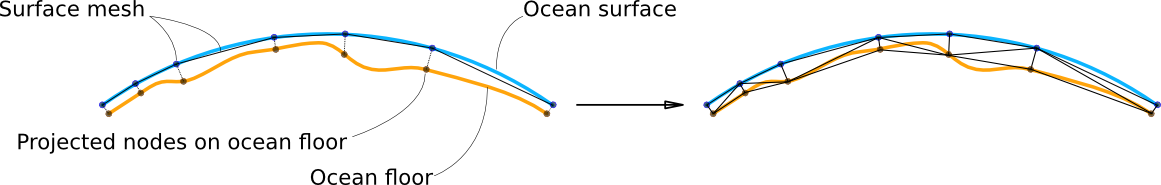
\includegraphics[width=1.0\textwidth]{../figures/mesh_extrusion.png}
\end{figure}
\end{frame}

\begin{frame}{Meshing realistic ocean domains: Key points}
\begin{itemize}
   \item A Gmsh user typically has to specify two essential parts:
   \begin{itemize}
      \item[$\circ$] Domain shape.
      \item[$\circ$] Characteristic element size.
   \end{itemize}\vspace{20pt}
   \item The geometry is very complex, boundaries are fractal--like
   \item Ideal characteristic element size can also be dependent on many parameters, for example:
   \begin{itemize}
       \item[$\circ$] Depth
       \item[$\circ$] Ocean floor topography
       \item[$\circ$] Explicit requirement in order to resolve tidal turbine array, etc.
   \end{itemize}
\end{itemize}
%\begin{figure}[htbp!]
% \centering
%  \includegraphics[width=0.27\textwidth]{../figures/UK_bathymetry_metric.png}
%\end{figure}
\end{frame}

\begin{frame}{Meshing realistic ocean domains: Challenges}
A simple CAD engine is insufficient:
\begin{itemize}
   \item Shorelines are geometrically very complex.
   \item The Gmsh GSHHS plug--in fits a spline through the GSHHS points, leading to intersecting shorelines (support for Gmsh GSHHS plugin now dropped).
   \item Drawing arbitrary lines as open boundaries --e.g. contour at a given depth-- not easily done.
\end{itemize}
\begin{figure}[htbp]
 \centering
  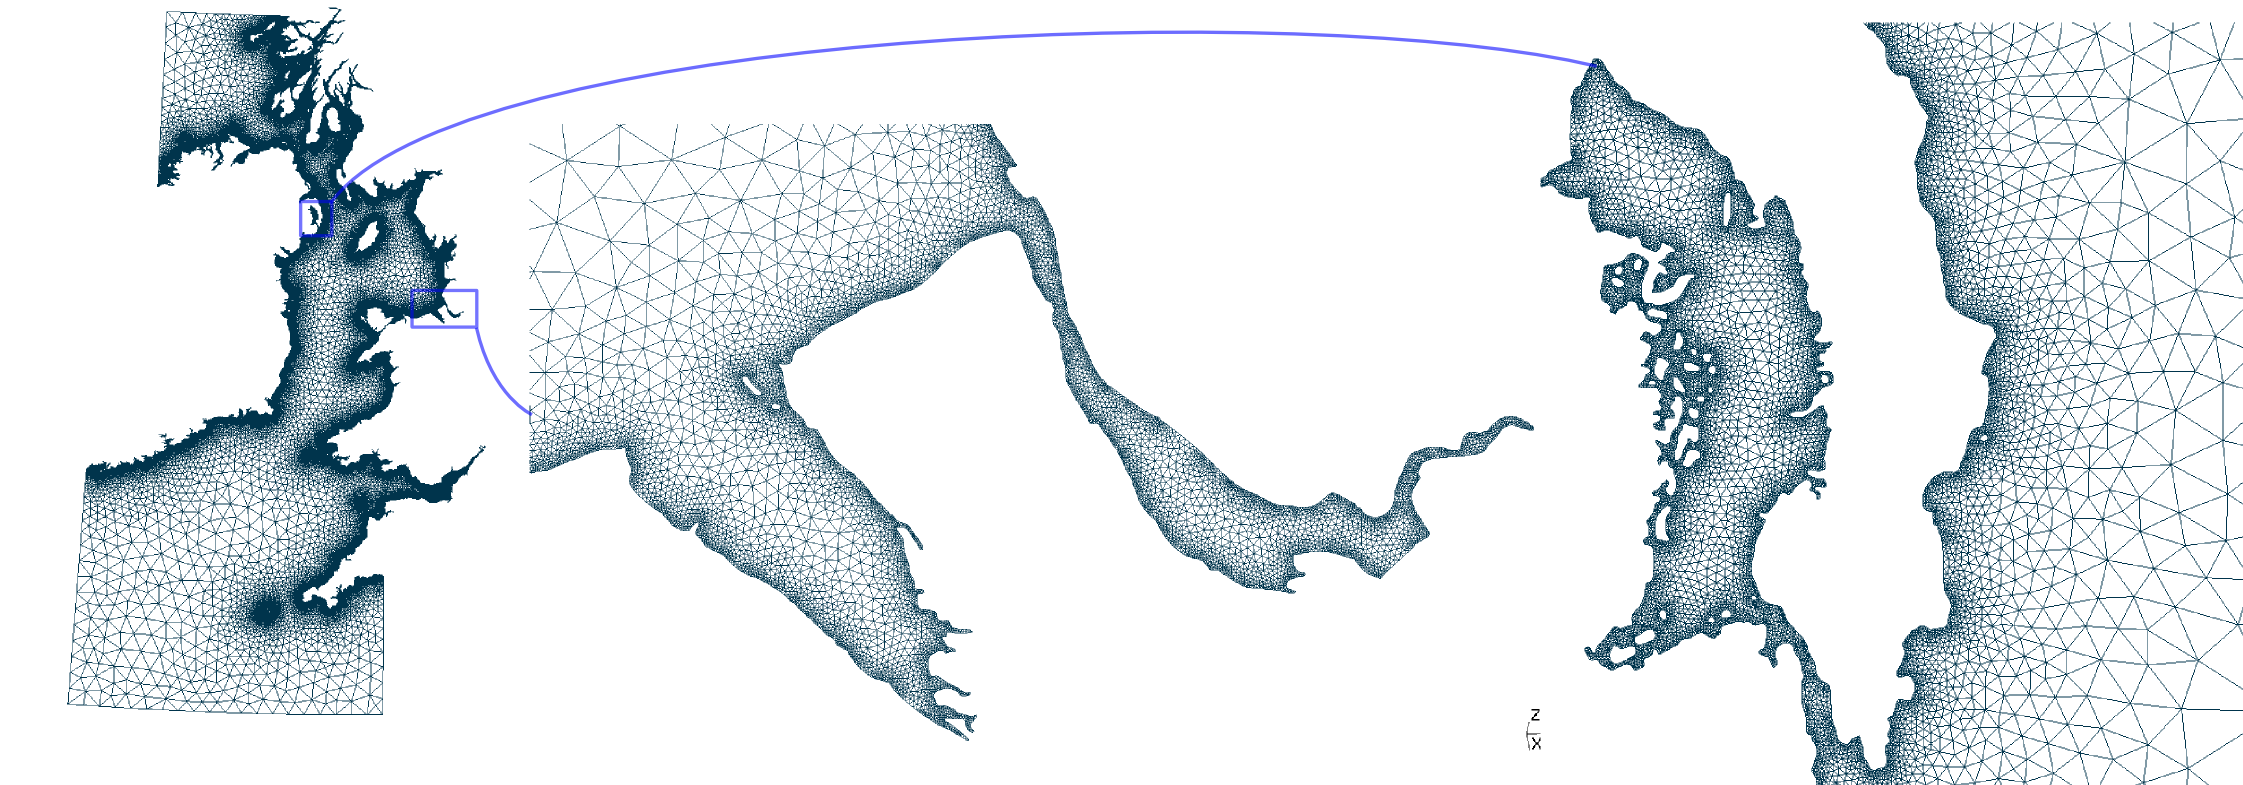
\includegraphics[width=1.00\textwidth]{../figures/UKwc_mesh_with_details/UK_west_coast_with_details}
  \caption{Mesh of the Irish Sea and surrounding seas, with highlighted details}
  \label{fig:IrishSeaMesh}
\end{figure}
\end{frame}

\begin{frame}{More challenges}
The spatial variation of the mesh element size could be complex:
%\begin{columns}
%\column{0.5\textwidth}
\begin{itemize}
   \item Mesh element size must usually be fine near the coastlines to capture their structure.\\[15pt]
   \item Mesh element size must usually be fine in areas of steep ocean floor topography and in shallow areas: Not easily done with current approach.
\end{itemize}
%\column{0.5\textwidth}
%\begin{figure}[htbp!]
% \centering
%  \includegraphics[width=1.00\textwidth]{../figures/UK_bathymetry_metric.png}
%\end{figure}
%\end{columns}
\end{frame}

\begin{frame}{Meshing realistic domains -- Our proposed approach}
Use Geographical Information Systems to extract domain boundaries and prescribe mesh metric size.
\begin{itemize}
   \item Existing GIS software capable of reading databases in popular formats.
   \item Capability of extracting contours from field-type databases is usually available. ($\rightarrow$domain boundaries)
   \item Capability of generating field-type databases is usually available. ($\rightarrow$mesh size metric)
\end{itemize}
\end{frame}

\begin{frame}{Further reading}
\begin{thebibliography}{9}

  \bibitem{presentDocumentPdf}
  AMCG, 
  \emph{The present slides},
  accessible via \href{https://github.com/FluidityProject/training}{GitHub} and \href{http://figshare.com/s/0dbd16a2635b11e4a71206ec4b8d1f61}{Figshare}.

  \bibitem{gmsharticle}
  C. Geuzaine and J.-F. Remacle,
  \emph{Gmsh: a three-dimensional finite element mesh generator with built-in pre- and post-processing facilities.}
  International Journal for Numerical Methods in Engineering,
  Volume 79, Issue 11,
  pages 1309-1331, 2009.

  \bibitem{gmshwebsite}
  C. Geuzaine and J.-F. Remacle,
  \emph{Gmsh Reference Manual.}.
  Available at
  \url{http://geuz.org/gmsh/\#Documentation}.

  \bibitem{amcg-gmsh-tutorial}
  A. Avdis and S.L.Mouradian,
  \emph{A Gmsh tutorial},
  accessible via \href{GitHub}{https://github.com/FluidityProject/training} and \href{Figshare}{}.

  \end{thebibliography}

\end{frame}

\begin{frame}{Questions?}
\begin{center}
\vfill
AMCG:\\
\url{http://amcg.ese.ic.ac.uk/}\\[15pt]
Fluidity:\\
\url{http://fluidityproject.github.io/}\\[15pt]
Fluidity code on GitHub:\\
\url{https://github.com/FluidityProject/fluidity}
\url{https://github.com/FluidityProject}\\[15pt]
Fluidity wiki:\\
\url{https://github.com/FluidityProject/fluidity/wiki}
\end{center}
\end{frame}

\end{document}

